\documentclass[border=0.25cm]{standalone}
\usepackage{tikz}
\usepackage{xcolor}
\tikzset{
    point/.style={ fill }
}

\begin{document}
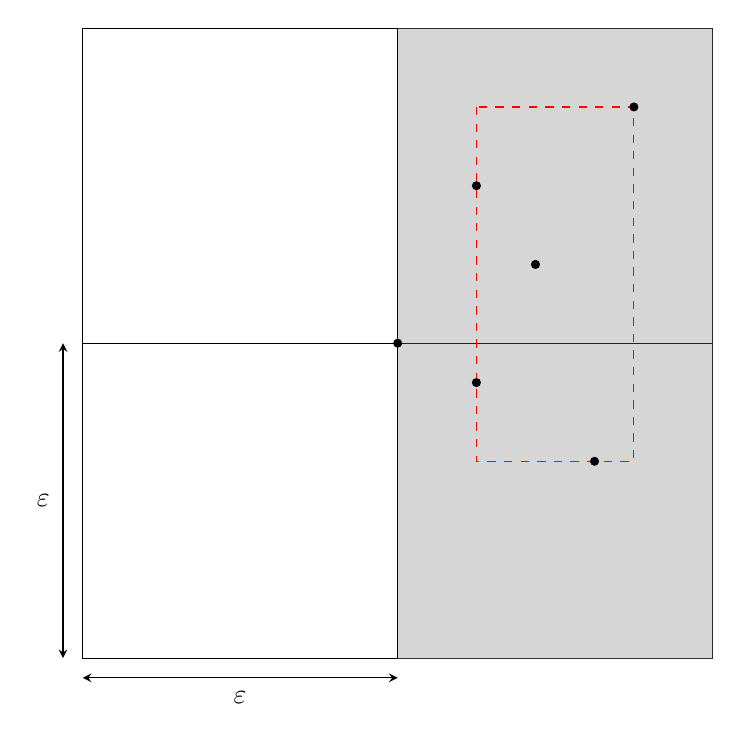
\begin{tikzpicture}
\coordinate (O) at (0,0);
\coordinate (A) at (0,4);
\coordinate (B) at (8,0);
\coordinate (C) at (0,8);
\coordinate (D) at (4,0);
\coordinate (E) at (4,4);
\coordinate (F) at (4,8);
\coordinate (G) at (8,8);
\coordinate (H) at (8,4);

\draw[] (O) -- (A) -- (E) -- (D) -- cycle;
\draw[] (A) -- (E) -- (F) -- (C) -- cycle;
\draw[fill=black!20,opacity=0.8] (E) -- (H) -- (G) -- (F) -- cycle;
\draw[fill=black!20,opacity=0.8] (D) -- (B) -- (H) -- (E) -- cycle;

\draw[stealth-stealth] (-0.25, 0) -- (-0.25, 4);
\node[] at (-.5,2) {$\varepsilon$};
\draw[stealth-stealth] (0, -0.25) -- (4, -0.25);
\node[] at (2,-.5) {$\varepsilon$};

\coordinate (B0) at (5,7);
\coordinate (B1) at (5,2.5);
\coordinate (B2) at (7,2.5);
\coordinate (B3) at (7,7);
\draw[dashed, red] (B0) -- (B1) -- (B2) -- (B3) -- cycle;

\coordinate (P0) at (4,4); \draw[point] (P0) circle (0.05);
\coordinate (P1) at (5,3.5); \draw[point] (P1) circle (0.05);
\coordinate (P2) at (5.75,5); \draw[point] (P2) circle (0.05);
\coordinate (P3) at (6.5,2.5); \draw[point] (P3) circle (0.05);
\coordinate (P4) at (5,6); \draw[point] (P4) circle (0.05);
\coordinate (P5) at (7,7); \draw[point] (P5) circle (0.05);

\end{tikzpicture}
\end{document}
